\documentclass[lettersize,journal]{IEEEtran}
\usepackage{amsmath,amsfonts}
\usepackage{algorithmic}
\usepackage{algorithm}
\usepackage{array}
\usepackage[caption=false,font=normalsize,labelfont=sf,textfont=sf]{subfig}
\usepackage{textcomp}
\usepackage{stfloats}
\usepackage{url}
\usepackage{verbatim}
\usepackage{graphicx}
\usepackage{lipsum}
\usepackage{cite}
\hyphenation{op-tical net-works semi-conduc-tor IEEE-Xplore}
% updated with editorial comments 8/9/2021

\begin{document}

\title{DNN Model Placement for Edge Intelligence}

\author{Convex Optimization 2 Course Project, Nima Samadi, Mohammad Javad Mohammadi}

% The paper headers
%\markboth{Journal of \LaTeX\ Class Files,~Vol.~14, No.~8, August~2021}%
%{Shell \MakeLowercase{\textit{et al.}}: A Sample Article Using IEEEtran.cls for IEEE Journals}

%\IEEEpubid{0000--0000/00\$00.00~\copyright~2021 IEEE}
% Remember, if you use this you must call \IEEEpubidadjcol in the second
% column for its text to clear the IEEEpubid mark.

\maketitle

\begin{abstract}
Edge Intelligence (EI) has emerged as a promising area in recent years. In order to mitigate some of the challenges associated with using AI in cloud servers, EI utilizes edge computing to deliver AI services to users. The dominant approach to creating AI services is deep neural networks (DNN) which have shown significant results in computer vision, language processing, robotics, etc., tasks. In the cloud, these models run on powerful servers, but they are slow to respond, have privacy concerns, and have low reliability. EI can help to overcome these obstacles. However, edge servers are typically constrained in terms of processing power and energy. Therefore, special care must be taken to deploy DNN models on edge servers. Our purpose in this project is to partition DNN models and place each part either on edge servers or the user device. We use optimization approaches to analyze this problem. 
\end{abstract}

\begin{IEEEkeywords}
Edge intelligence, Model placement, Neural network, Convex optimization
\end{IEEEkeywords}

\section{Introduction}

Deep Neural Networks (DNNs) have become increasingly popular as the core machine learning technique in many fields, such as speech recognition, image classification, translation, language modeling, and video captioning. 
DNNs are widely used to perform these tasks due to their high accuracy and adaptability. The training of model parameters requires massive amounts of data that can only be achieved with powerful hardware and adequate time. Additionally, since neural networks are widely used, it is essential to research how to utilize and train them optimally.

One solution to tackle this issue is cloud computing, which undoubtedly poses real challenges to network capacity and the computing power of cloud computing infrastructures. Also, many new applications such as cooperative autonomous driving, are sensitive to delay requirements that the cloud infrastructures would have difficulty meeting since they may be far from the users. 

Another solution that has become a hot topic in the computation context is edge computing. Edge computing has many benefits, such as alleviating the network traffic load as less data is exchanged with the cloud compared to the cloud-only scenario. Furthermore, services hosted at the edge can substantially reduce the delay time of data transmissions and improve the response time. The users' privacy is also enhanced as the private data is stored locally on the edge or user devices instead of cloud servers. The hierarchical computing architecture provides more reliable computation, and finally, edge computing can promote the pervasive application of DNNs.
 
Cloud computing and edge computing aren't mutually exclusive, and that's crucial to understand. In other words, edge computing complements and extends cloud computing. High processing power, giant storage, and data backup are some of the capabilities of cloud servers that edge servers lack. On the contrary, low latency, privacy assurance, and real-time processing are some of the capabilities of edge servers that cloud servers lack. The combination of these computation paradigms enables cumulating advantages of each and reduces the disadvantages.
 
Edge intelligence (EI) refers to the data analysis and development of solutions at the site where data is generated. Indeed, edge intelligence reduces latency, costs, and security risks, thus making the associated business more efficient. In other words, edge devices help DNN models to be trained and deployed more efficiently. 

EI is used for optimizing the costs associated with fleet management. Industrial manufacturers use EI to improve real-time data processing. Software companies use EI to develop personalized data-driven experiences to attract their customers. Multiple System Operators (MSOs) use EI to maximize the lifetime value of their subscribers.

\section{Related work}
Throughout this section, we review some research related to mobile edge intelligence, server selection, and model placement.

Edge intelligence (EI), the integration of mobile edge computing (MEC) and AI technologies, has recently emerged as a promising paradigm to support computation-intensive AI applications at the network edge \cite{9442308}.
An edge-based MEC network with multiple edge servers is studied in \cite{8737385} to maximize the number of computing offloading requests under edge storage, computation, and communication constraints. To cope with the unknown and fluctuating service demand,\cite{8509631} proposed an online learning algorithm to optimize spatial-temporal dynamic service placement decisions among multiple edge servers to minimize the computation delay. Considering parallel computing at both cloud and edge servers, \cite{xu2018joint} and \cite{chen2019collaborative} studied collaborative service placement and computation offloading to minimize the computation latency.

Due to resource limitations on the edge server, server selection has received considerable attention in recent years \cite{9599379}. 
Researchers have proposed techniques to achieve optimal goals when selecting servers, such as minimizing the average delay \cite{8972932},
maximizing the resources utilization efficiency \cite{8823875}, minimizing energy consumption \cite{li2020energy} and etc.

In some research like \cite{liu2021deep}, the continuous server selection problem is modeled as a Markov Decision Process (MDP). Deep Reinforcement Learning (DRL) techniques are proposed to address the issue of dealing with highly dynamic environments modeled by MDP. The time and computations necessary to train DRL models are substantial, even though these methods can reach good solutions.  Additionally, since DRL models need to be trained periodically, this method cannot be used in many situations, especially in real-time applications. 

\section{Methodology}
\subsection{introduction}
We analyze this problem from an optimization point of view. This technique is used in \cite{DBLP:journals/corr/abs-2006-16423}, \cite{9527097}, and \cite{9512507} articles. Every DNN model can be thought of as a directed graph in which nodes are operations and edges are data (tensor in software terms). The direction of the edge shows the dependency between nodes. One can model this graph with three possible granularities: (a) neuron, (b) operation, and (c) layer. With neuron granularity, the dimension of the problem is quite high and the number of connections between neurons prevents partitioning the graph effectively. Layer abstraction, however, results in a small graph, which makes parallelization difficult. Therefore, we use operation granularity in this project. 

Placement problems consist of two subproblems: (a) graph partitioning and (b) task assignment. Graph partitioning requires segmentation points that enable parallel execution of each subgraph and minimizes dependency between subgraphs. When subgraphs are created, they must be processed on the user device or an edge server. This task assignment problem can be solved via optimization techniques.

Let $G(V, E)$ to be the model graph and $\mathcal{P} = \{p_1, p_2, \cdots p_k\}$ be the list of $k$ processors. A model placement means finding the set of $\{(p_1, s_1), (p_2, s_2), \cdots, (p_k, s_k)\}$, where each $s_i$ is a subpraph and all $s_i$ form a partition of graph. In other words, $\bigcup s_i = V$, and $\bigcap s_i = \emptyset$. Among all feasible points, we choose one that minimizes total latency of model execution. The objective function depends on how latency is defined and will be the subject of project itself.

\subsection{Formulation}
\begin{enumerate}
\item{model description}
\item{objective function}
\item{constraints}
\item{conversion and discussion}
\end{enumerate}
\begin{figure*}[!t]
\centering
\subfloat[]{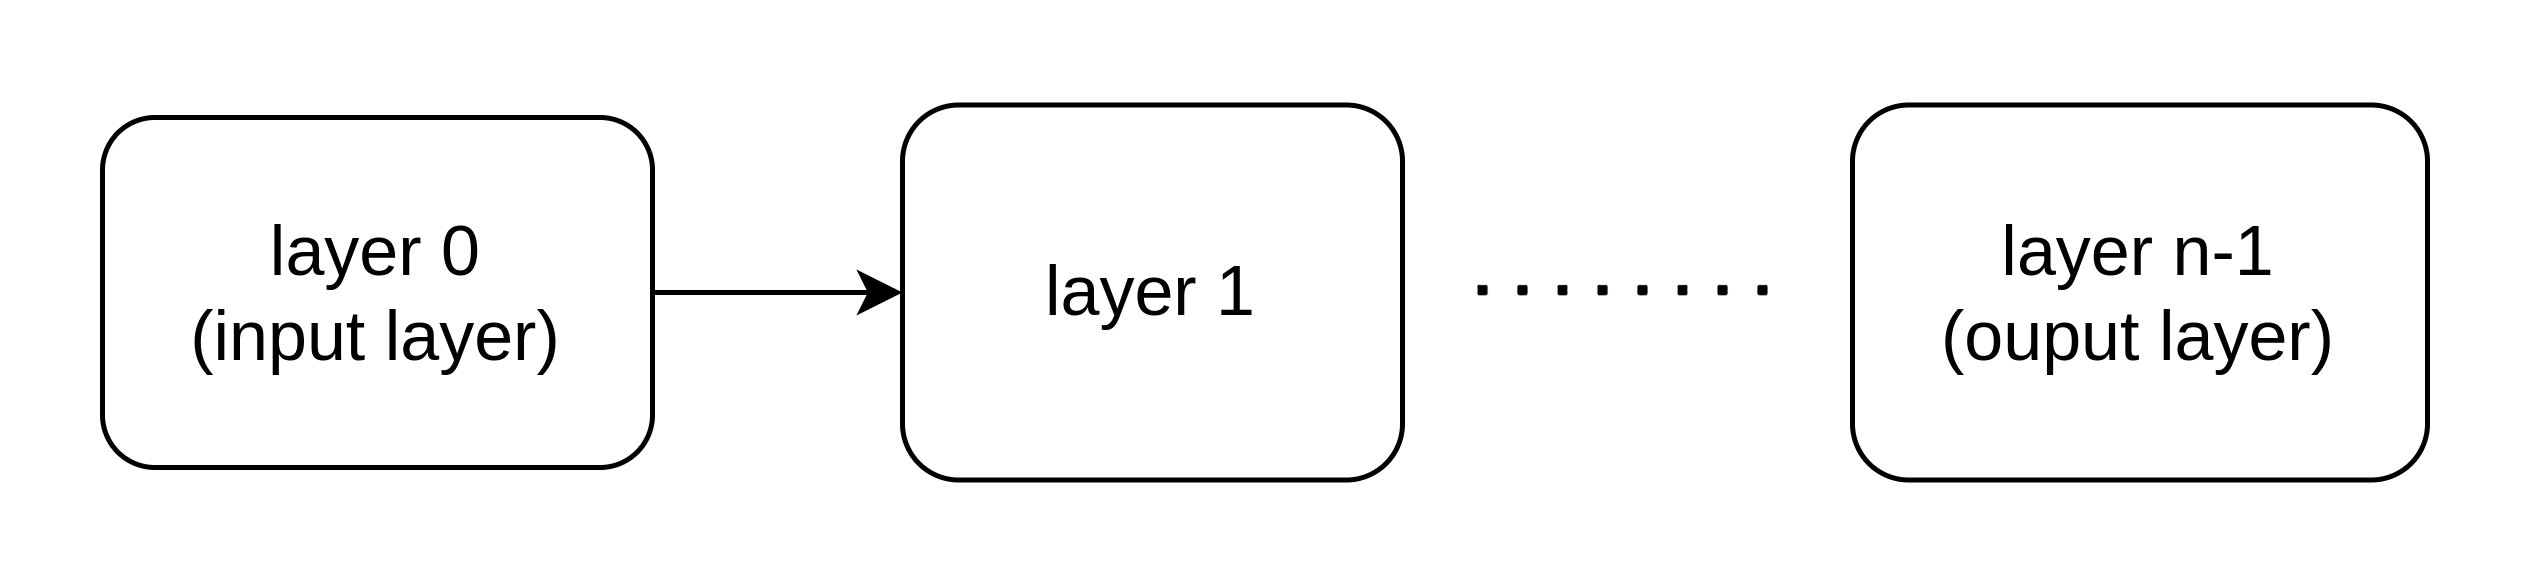
\includegraphics[width=3in]{assets/layers.png}%
\label{fig_first_case}}
\hfil
\subfloat[]{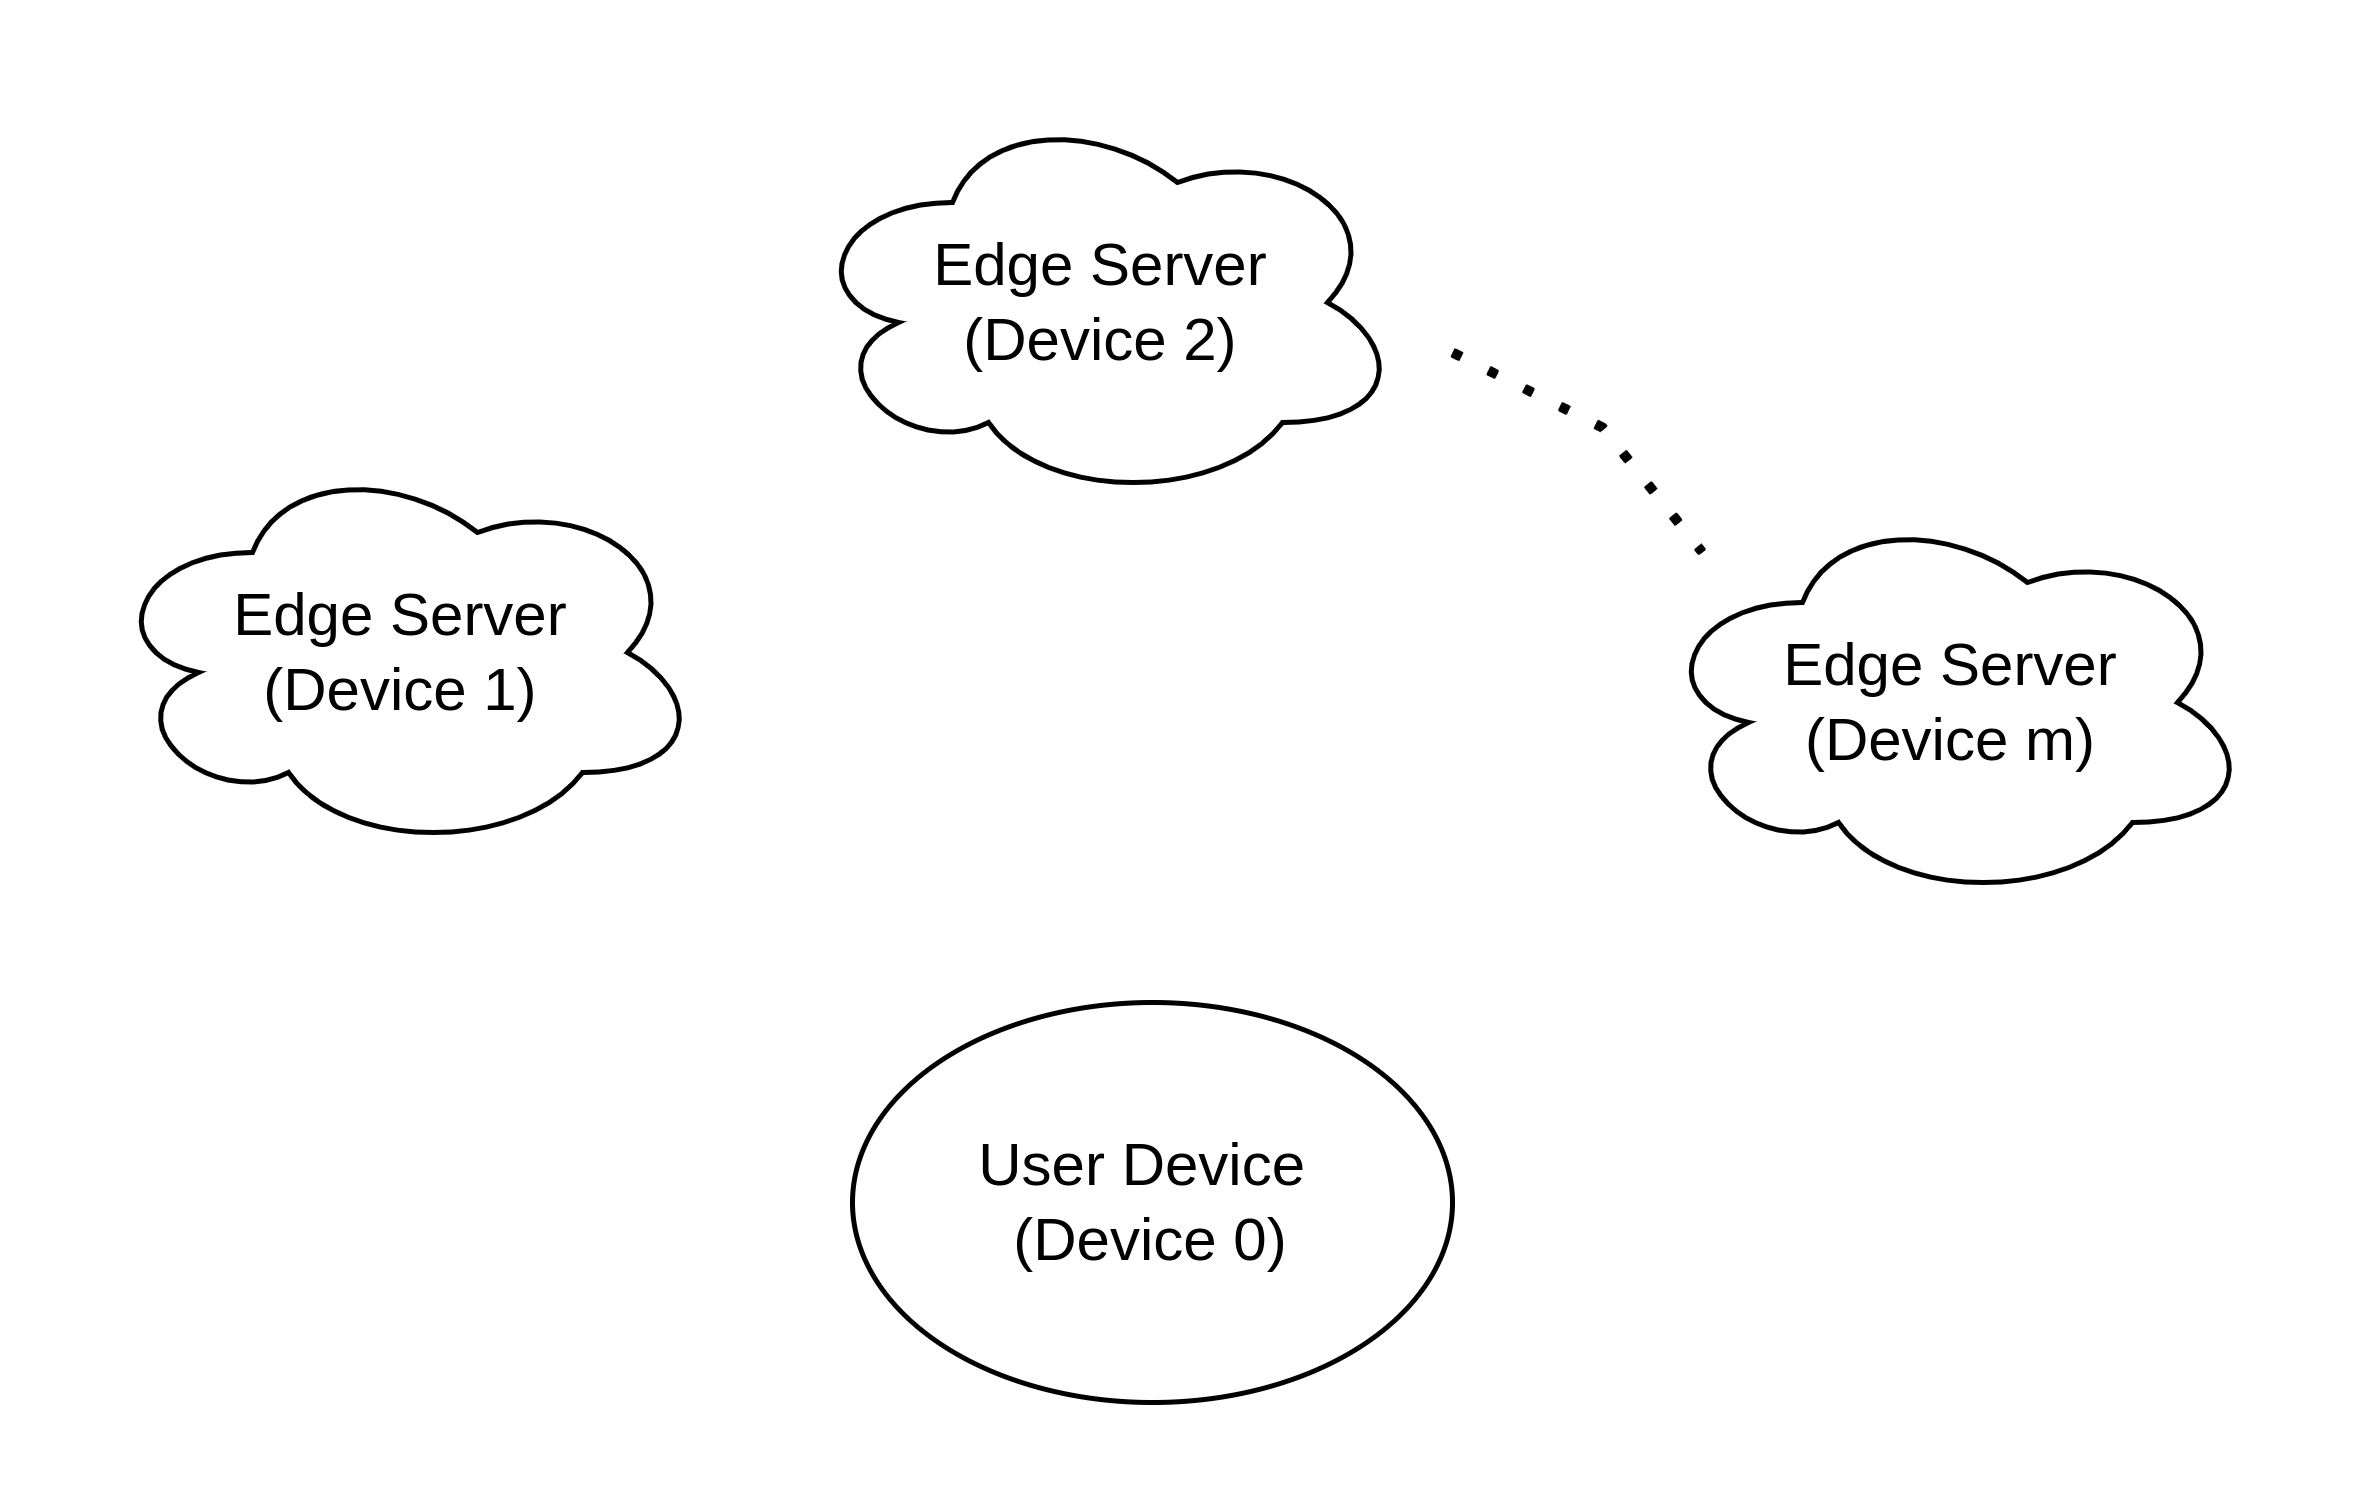
\includegraphics[width=3in]{assets/devices.png}%
\label{fig_second_case}}
\caption{System model. (a) Neural network architecture. (b) Computation recources.}
\label{fig_sim}
\end{figure*}

\subsection{Simulation}
\begin{enumerate}
\item{how to solve?}
\item{mosek}
\item{simulation with cvxpy}
\item{some results}
\end{enumerate}
\section{Conclusion}
In this project we investigated a simple

{\appendix[Complete Matrix Representation]
Here we will show complete matrix repr.
}

\bibliographystyle{IEEEtran}
\bibliography{IEEEabrv,citation.bib}
\end{document}
